\documentclass{article}
\usepackage{graphicx}
\usepackage{caption}
\usepackage{subcaption}
\usepackage[paper=a4paper,margin=1in]{geometry}
\usepackage[fontsize=12pt]{fontsize}
\usepackage[hidelinks]{hyperref}
\usepackage{amsmath}

\title{Math 475 -- Project 1 \\ Bobcat Population}
\author{Jackson Brienen}
\date{October 8 2025}

\begin{document}

\maketitle

\section{Introduction}
In this paper we discuss how we can model bobcat populations under a variety of environmental conditions and external manipulations (hunting and introduction). While there are a variety of modeling techniques that can be used for populations we focus on using a basic exponential model. With this come a variety of assumptions:

\begin{enumerate}
    \item There is no carrying capacity/ maximum population.
    \item The growth rate of the population is always constant, i.e. the growth rate in the first year will be the same as the hundredth year, and thousandth year, and so on.
    \item We assume, in most cases, that fractional populations are valid. While one half of a bobcat does not usually make sense, for the sake simplicity we will allow it to be the case unless we explicitly say we use integer based populations.
    \item All births and deaths happen at the end of a year/ start of a new year.
    \item All time increments, denoted $t$ throughout the paper, are integers greater than or equal to zero.
\end{enumerate}

This paper will be divided into three main topics. First, the analysis of the basic model under three different growth rates in both the long and short term. Second, we will how the model changes when hunting is introduced and devising a strategy to meet a stable population with hunting. Third and last, we will analyze how the model changes when external introduction is used along with devising a strategy to meet a stable population with introduction.

% \section{Methods} % maybe add this? I feel like the whole paper is going to describe the methods we use, so I don't think this is that needed.

\section{Basic Growth}
This section discusses the basic growth model which we use throughout this paper. We start with a very basic recursive function $P(t)$ which takes our previous population $P(t-1)$ and adds the annual change to the population $rP(t-1)$, where $r$ is some growth rate. This simplifies to \autoref{eq:basic-recursive-exponential}.

\begin{equation} \label{eq:basic-recursive-exponential}
    P(t) = (r+1)P(t-1)
\end{equation}

Previously we mentioned we were using an exponential model, yet this recursive formula does not look exponential. While it might not be immediately obvious, we can solve the recurrence for its closed form expression.

\begin{align*}
    P(t) &= (r+1)P(t-1) & P(t-1) &= (r+1)P(t-2) \\
    P(t) &= (r+1)\left((r+1)P(t-2)\right) & P(t-2) &= (r+1)P(t-3) \\
    P(t) &= (r+1)\left((r+1)\left((r+1)P(t-3)\right)\right) & P(t-3) &= (r+1)P(t-4) \\
    &\phantom{x}\vdots \\
    P(t) &= (r+1)^tP(0)
\end{align*}

In this closed form we can see clearly that this is in fact an exponential model. We can see this exponential nature by graphing our model. There are three growth rates based on environmental conditions, $1.676\%$ in the best case, $0.549\%$ in moderate cases, and $-4.5\%$ in the worst case, we will look at these when the starting population is $100$.

\begin{figure}[h]
    \centering
    \begin{subfigure}{.5\textwidth}
        \centering
        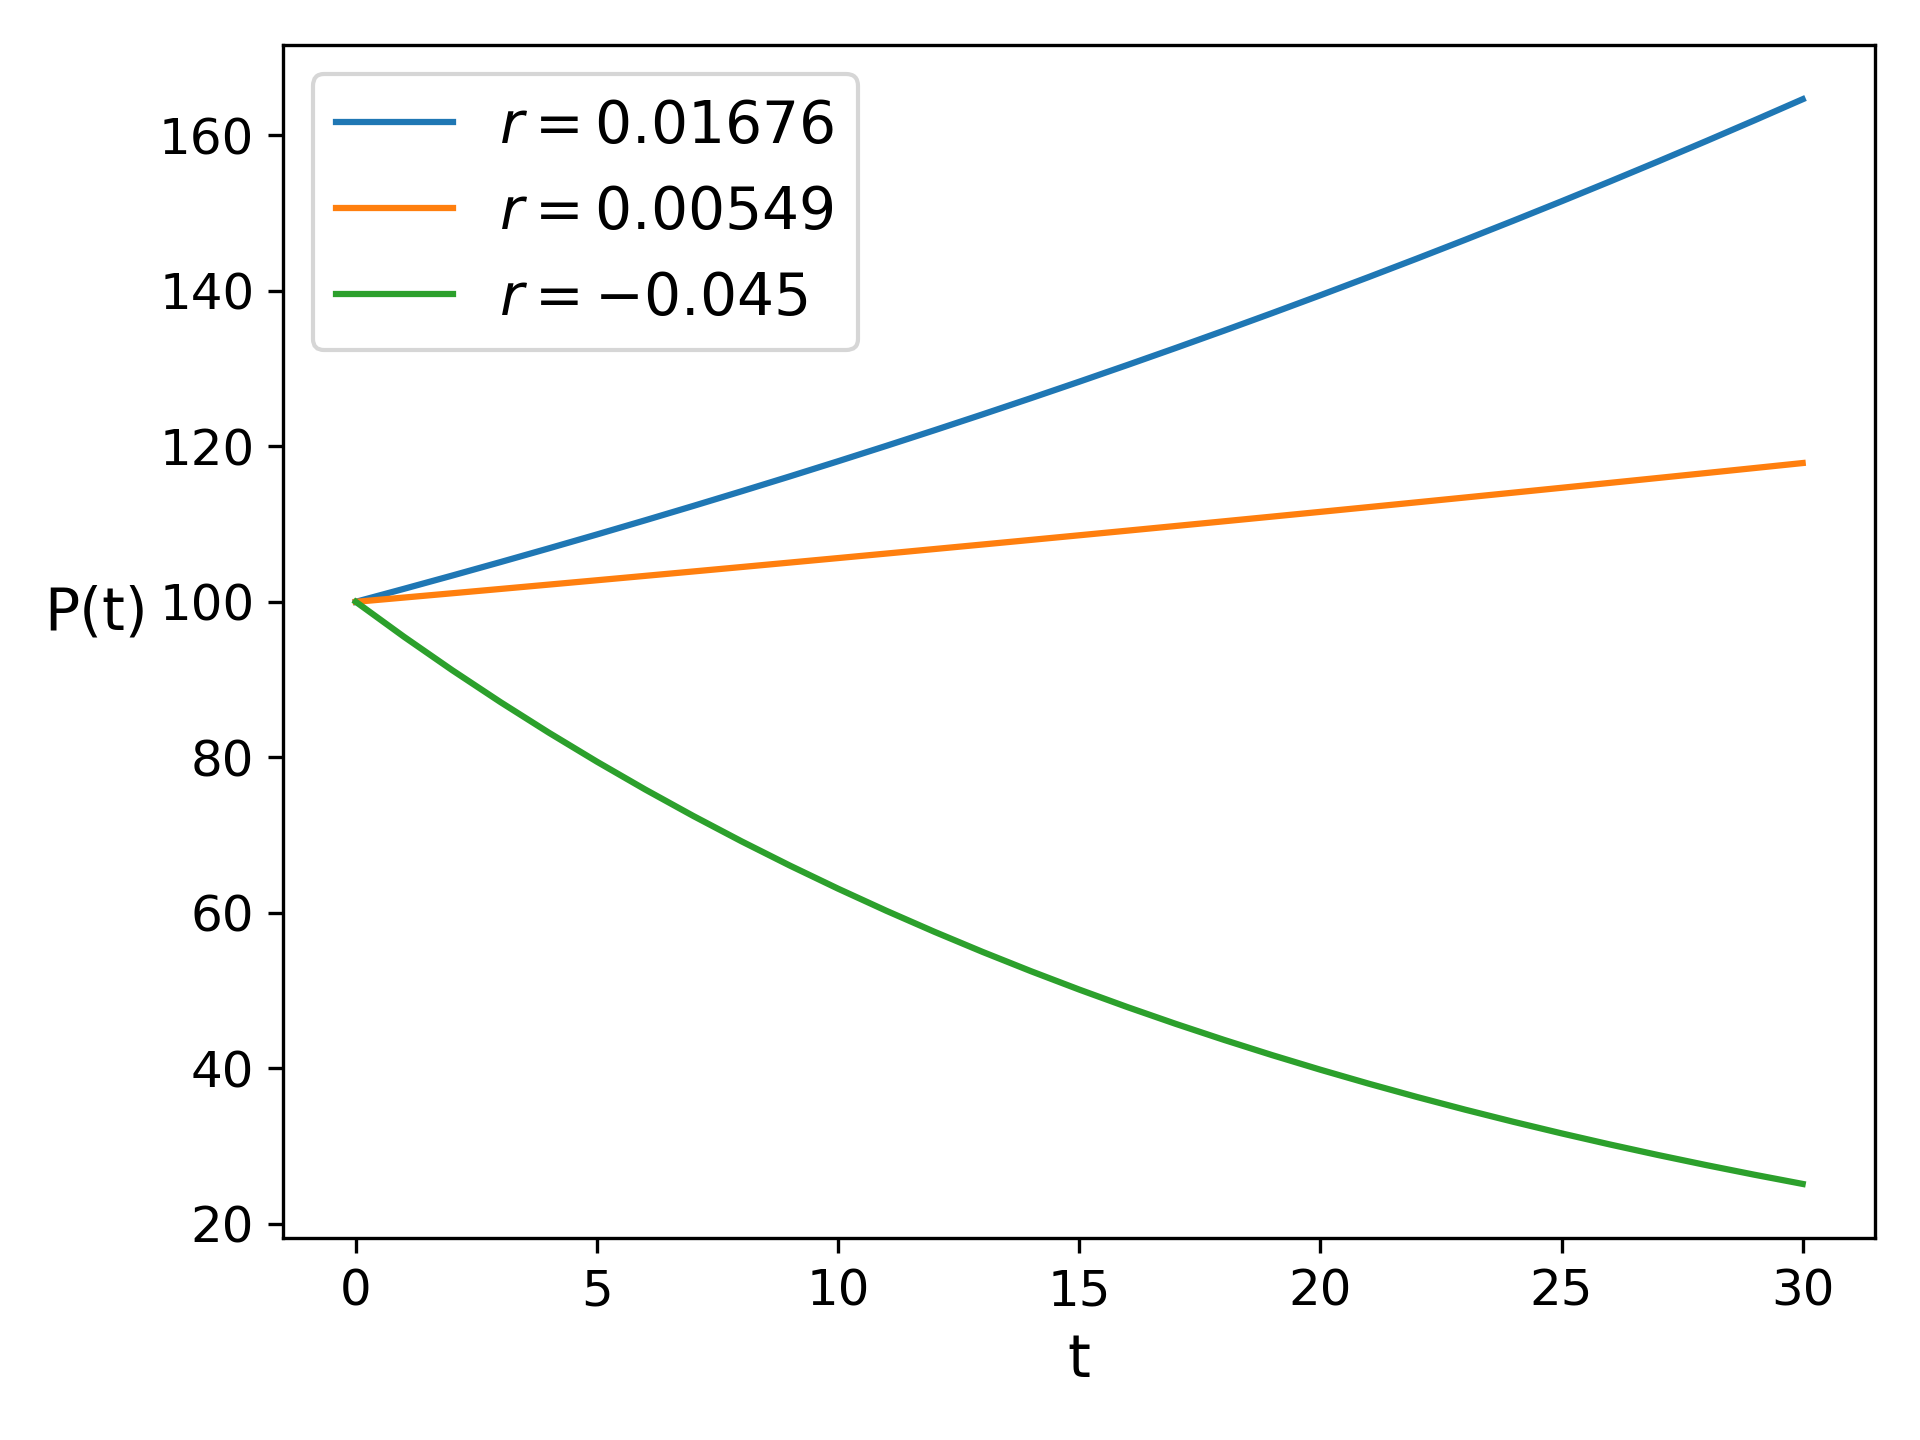
\includegraphics[width=.95\linewidth]{./basic/short_term.png}
        \caption{Bobcat Population over 30 Years}
        \label{fig:basic-short-term}
    \end{subfigure}%
    \begin{subfigure}{.5\textwidth}
        \centering
        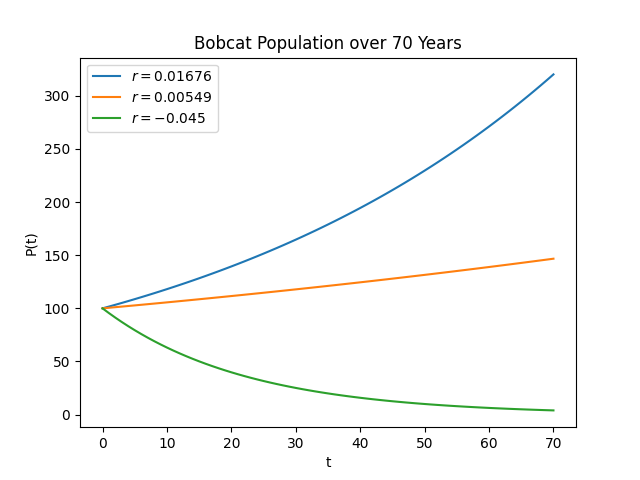
\includegraphics[width=.95\linewidth]{./basic/long_term.png}
        \caption{Bobcat Population over 70 Years}
        \label{fig:basic-long-term}
    \end{subfigure}
    \caption{Bobcat populations in the short (30 year) and long (70 year) term. Using \autoref{eq:basic-recursive-exponential} with $P(0) = 100$, and three different growth rates, $r$, being $1.676\%$, $0.549\%$, and $-4.5\%$.\protect\footnotemark{}}
    \label{fig:test}
\end{figure}

\footnotetext{\href{https://github.com/JacksonBrienen/CWU-Math475-Mathematical-Modeling/tree/project1/basic}{github.com/JacksonBrienen -- Graphs} \\ \phantom{111} \href{https://github.com/JacksonBrienen/CWU-Math475-Mathematical-Modeling/blob/project1/q1.py}{github.com/JacksonBrienen -- Code for Graphs}}

While in \autoref{fig:basic-short-term} it is difficult to see our exponential behavior in all cases except $r = -0.045$, it becomes obvious in \autoref{fig:basic-long-term}. In the case where $r = -0.045$, we know our function takes the form $P(t) = (1-0.045)^tP(0)$, which means $0.955$ will be multiplied together $t$ times, to get our population for any given $t$. Since $0.955 < 1$, our population will be decreasing, as we can see in both figures. We also know that, while population will continue to get smaller as $t \rightarrow \infty$, it will never reach zero. This behavior is seen in \autoref{fig:basic-long-term} as we see the line become asymptotic to zero.

For $r = 0.01676$ (in blue) and $r = 0.00549$ (in orange) we see similar behavior, since in both cases $r + 1 > 1$ we know the population will always be increasing. We know that there is nothing in our model to stop this growth, so as $t \rightarrow \infty$ $P(t) \rightarrow \infty$, but at different rates depending on $r$. This is highlighted in the figures as both lines go upwards in similar manners, but at different rates.

This model appears to only have one point of stability, when $P(t) = 0$, and we only approach this stable point with negative $r$ values. We will discuss different methods of identifying stable, or fixed, points later in this paper.

\section{Hunting}
In the best of times ($r = 0.01676$) we would like to analyze how different forms of hunting can impact the population. We must modify \autoref{eq:basic-recursive-exponential} to account for both fixed amount hunting and fixed percentage hunting. For fixed amount hunting we will have some amount of bobcats $a$ which get hunted each year, seen in \autoref{eq:hunting-amount}. In this case $a$ will be negative, as we choose to allow this formula to work for both hunting bobcats and adding bobcats. The fixed percentage hunting works similarly, but uses a percentage $h$ of the population to be hunted, as seen in \autoref{eq:hunting-percentage}. Again $h$ will be negative in the case of hunting, but positive in the case of introduction.

\begin{equation}\label{eq:hunting-amount}
    P(t) = (r+1)P(t-1) + a
\end{equation}

\begin{align}\label{eq:hunting-percentage}
    P(t) &= (r+1)P(t-1) + hP(t-1) \nonumber \\
    P(t) &= (r+h+1)P(t-1)
\end{align}

Finding the closed form for each of these can allow us to better understand their behavior. The closed form of \autoref{eq:hunting-percentage} can be found the same as before, as the only thing that has changed is $(r+1)$ has become $(r+h+1)$, so our closed form will be \autoref{eq:hunting-percentage-closed}. \autoref{eq:hunting-amount} is slightly more complicated as it includes a new term, we can attempt to solve it in the same manner.

\begin{equation}\label{eq:hunting-percentage-closed}
    P(t) = (r+h+1)^tP(0)
\end{equation}

\begin{align*}
    P(t) &= (r+1)P(t-1) + a & P(t-1) = (r+1)P(t-2) + a \\
    P(t) &= (r+1)((r+1)P(t-2) + a) + a & P(t-2) = (r+1)P(t-3) + a \\
    P(t) &= (r+1)((r+1)((r+1)P(t-3) + a) + a) + a & P(t-3) = (r+1)P(t-4) + a \\
    &\phantom{x}\vdots \\
    P(t) &= (r+1)^tP(0) + \sum_{k=0}^{t-1}(r+1)^ka
\end{align*}

In this case we are left with the expected exponential term from \autoref{eq:basic-recursive-exponential}, but we also have a summation term. This term can be easily simplified using the geometric series formula, seen in \autoref{eq:geometric-series-formula}. Giving us a final closed from of \autoref{eq:hunting-amount-closed}.

\begin{equation}\label{eq:geometric-series-formula}
    \sum_{k=0}^{n-1}cx^k=\frac{c(x^n-1)}{x-1}
\end{equation}

\begin{equation}\label{eq:hunting-amount-closed}
    P(t) = (r+1)^tP(0) + a\frac{(r+1)^t-1}{r}
\end{equation}

% TODO: Finish this section

\section{Population Introduction}
    
\end{document}